\section{Resultados y Discusión}

Entre los resultados obtenidos, primero se comparó el ajuste de la subrogación del modelo con respecto a los datos del steptest. Posteriormente se realizó una evaluación del control por medio de los datos obtenidos en la co-simulación de Simulink y Aspen Plus Dynamics por métodos gráficos y los índices de rendimiento presentados anteriormente.

\subsection{Subrogación de modelos}

Los modelos subrogados se realizaron a partir de la consideración de dos entradas; la potencia del rehervidor y la relación de reflujo, con una salida de temperatura de etapa. En el caso de la $T-101$, los modelos predicen la temperatura de la etapa 36, mientras que en la $T-102$ se encuentra la temperatura de la etapa 8. Esto considerando los perfiles de temperatura donde se determina que estas etapas son las de mayor sesibilidad \cite{ref10}. De esta manera se obtienen los 4 modelos porevaluar para las dos torres: ARX, ARMAX, SS y NLARX-SVM. Se evalúan métricas de ajuste del sistema, sin embargo, un perfecto acople no es necesario para la implementación del modelo en control predictivo. En la Tabla 2 se puede evidenciar el RMSE y el R2, los cuales presentan una pequeña mejora en el siguiente orden entre modelos: $SS<ARX<ARMAX< NARX-SVM$ para $T-101$ y $ARX<ARMAX<SS< NARX-SVM$ para $T-102$. No obstante, es importante recalcar el alcance de todos los metamodelos al representar la tendencia general.

\begin{figure}[htbp]
    \centering
    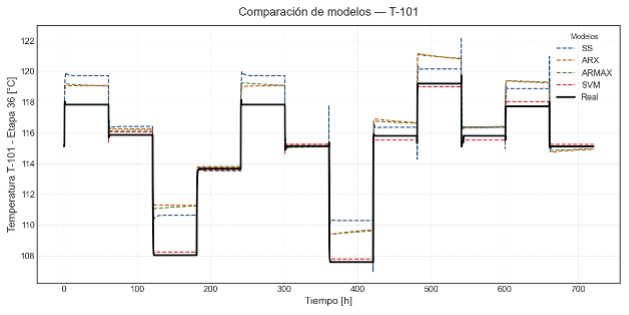
\includegraphics[width=0.6\textwidth]{figures/ModelosT101.png}
    \caption{Comparación de los modelos subrogados para el control de $T-101$}
    \label{fig:ModelosSubrogadosT101}
\end{figure}

\begin{figure}[htbp]
    \centering
    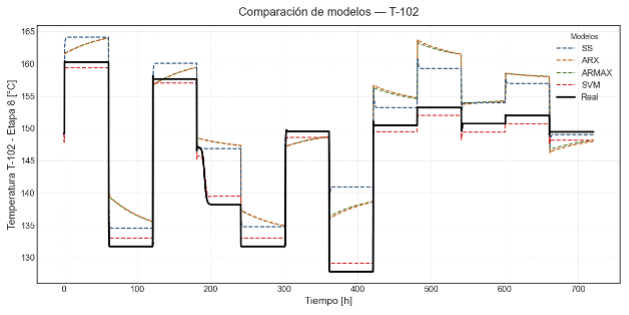
\includegraphics[width=0.6\textwidth]{figures/ModelosT102.png}
    \caption{Comparación de los modelos subrogados para el control de $T-102$}
    \label{fig:ModelosSubrogadosT102}
\end{figure}

\begin{table}[htbp]
\centering
\caption{Métricas de las subrogaciones de control}
\label{tab:ModelosR2}
\renewcommand{\arraystretch}{1.1}
\setlength{\tabcolsep}{6pt}
\begin{tabular}{l l c c}
\toprule
Columna & Modelo & RECM & $R^2$ \\
\midrule
T-101 & SS    & 1.4331 & 0.8327 \\
T-101 & ARX   & 1.4276 & 0.8340 \\
T-101 & ARMAX & 1.4073 & 0.8387 \\
T-102 & SS    & 5.4304 & 0.7232 \\
T-102 & ARX   & 5.7524 & 0.6894 \\
T-102 & ARMAX & 5.7294 & 0.6919 \\
\bottomrule
\end{tabular}
\end{table}

\FloatBarrier
\subsection{Control predictivo frente a perturbaciones}

Al obtener los modelos que relacionan las variables manipuladas con la variable controlada, es posible implementar el MPC y realizar pruebas de comportamiento frente a perturbaciones. Estas son un aumento del 8\% en ente. Teniendo en consideración la implementación de los modelos en el MPC, solo se realizó el control predictivo de los modelos lineales: ARX, ARMAX, SS. Los resultados comparativos se dividieron en tres partes, comenzando por los costos computacionales en la Tabla 4 que evalúan el tiempo de Simulink, el CPU utilizado por paso y la memoria RAM necesaria para la simulación. Comparando los tres modelos se evidencia que el costo de segundos en Simulink y milisegundos de CPU por paso es el menor para el modelo de espacio de estado, sin embargo, la memoria RAM es la mayor a comparación de los otros dos modelos. A pesar de esto, es posible observar que las diferencias entre costos computacionales no son amplias, por lo cual son necesarios más criterios para determinar el mejor modelo.


\begin{figure}[htbp]
    \centering
    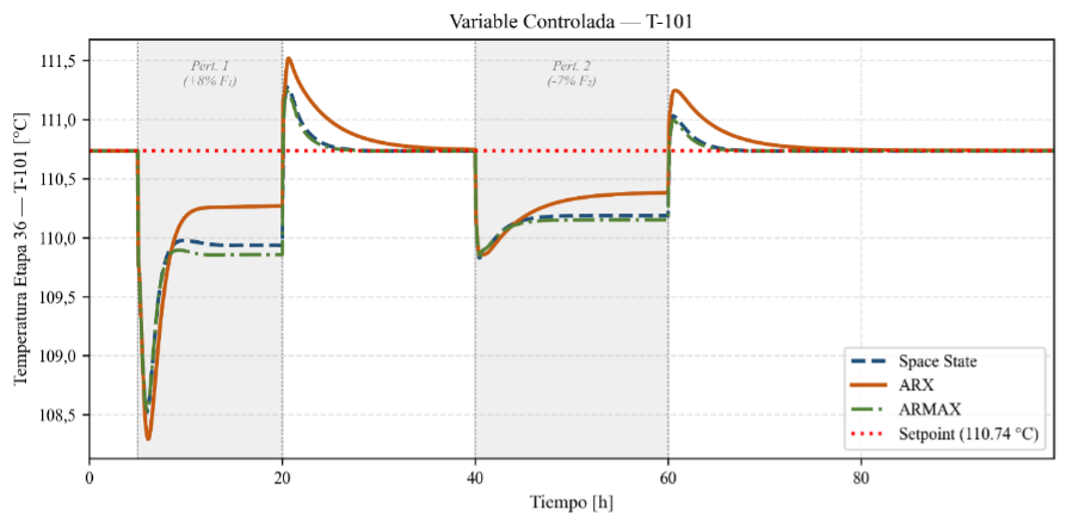
\includegraphics[width=0.6\textwidth]{figures/ControlT101.png}
    \caption{Comportamiento de la variable controlada en comparación con el valor nominal en la simulación de control $T-101$}
    \label{fig:ControlT101}
\end{figure}

\begin{figure}[htbp]
    \centering
    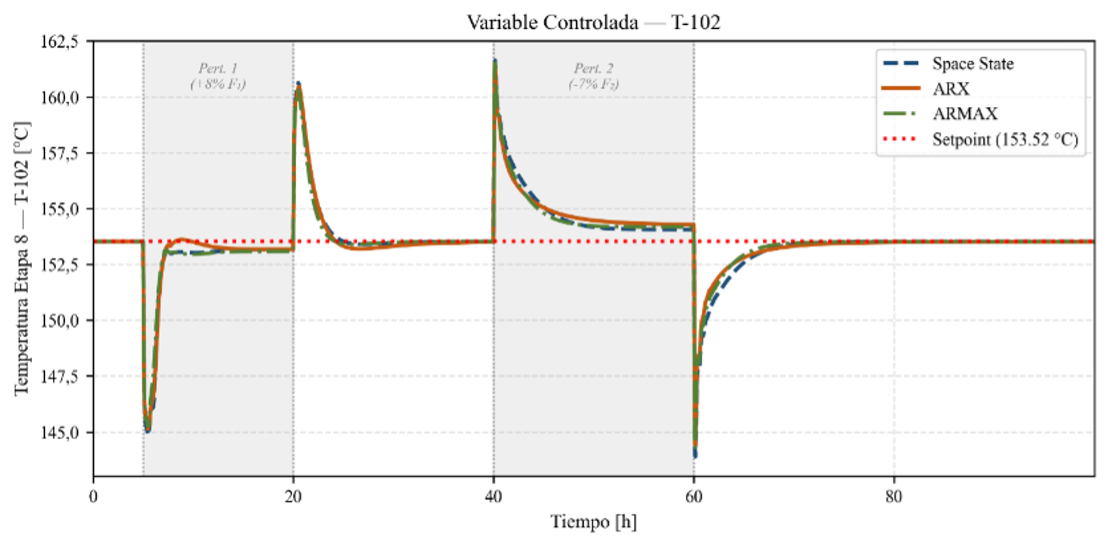
\includegraphics[width=0.6\textwidth]{figures/ControlT102.png}
    \caption{Comportamiento de la variable controlada en comparación con el valor nominal en la simulación de control $T-102$}
    \label{fig:ControlT102}
\end{figure}

Continuando con las métricas de control básicas, se comparan los tiempos de estabilización y el error con respecto al setpoint para las dos perturbaciones en cada modelo. En la Tabla 5 de denota que todos los metamodelos implementados en el MPC lograron alcanzar un error menor al 1\%, por lo que el objetivo de control de perturbaciones se alcanzó en los tres casos. De todos modos, se puede visualizar tanto en la tabla como en la Figura 4 y Figura 5 existen diferencias en el error y el tiempo de estabilización. En general, el modelo ARMAX generó una estabilización más rápida, de 6.7 horas aproximadamente, cercana a valores de literatura a comparación de los otros dos modelos. Sin embargo, el error en este metamodelo aumenta; caso contrario al modelo ARX, el cual tiene los errores más pequeños; incluso llegando a 0.2\% en $T-102$ para la primera perturbación; pero aumentando considerablemente el tiempo de estabilización. Debido a que ningún modelo es concluyente al compararlos por medio del tiempo y el error, es necesario utilizar criterios integrales de desempeño para determinar cuál realiza el mejor trabajo de control.

\begin{table}[htbp]
\centering
\caption{Costos computacionales}
\label{tab:CostosComputacionales}
\small
\begin{tabular}{lccc}
\toprule
Modelo & T. Simulink (s) & CPU/paso (ms) & RAM (MB) \\
\midrule
SS    & 1373.914 & 1136.406 & 6.156  \\
ARX   & 1425.248 & 1178.865 & 5.9959 \\
ARMAX & 1463.379 & 1210.405 & 6.0456 \\
\bottomrule
\end{tabular}
\end{table}

\begin{table}[htbp]
\centering
\caption{Métricas de las subrogaciones de control}
\label{tab:ControlMetrics}
\scriptsize
\setlength{\tabcolsep}{3pt}
\begin{tabular}{llcccccccc}
\toprule
Sistema & Modelo & P1 [°C] & P2 [°C] & SP [°C] & $er_1$ & $er_2$ & $t_1$ [h] & $t_2$ [h] \\
\midrule
T-101 & SS    & 109.93  & 110.19  & 110.73 & 0.72 & 0.49 & 7.42 & 6.42 \\
T-101 & ARMAX & 109.858 & 110.134 & 110.73 & 0.79 & 0.54 & 6.66 & 5.75 \\
T-101 & ARX   & 110.25  & 110.345 & 110.73 & 0.43 & 0.35 & 6.75 & 11.66 \\
T-102 & SS    & 153.17  & 154.05  & 153.52 & 0.23 & 0.35 & 10.83 & 13.91 \\
T-102 & ARMAX & 153.068 & 154.193 & 153.52 & 0.29 & 0.44 & 9.25 & 11.83 \\
T-102 & ARX   & 153.184 & 154.314 & 153.52 & 0.22 & 0.52 & 10.16 & 15.58 \\
\bottomrule
\end{tabular}
\end{table}

Con el objetivo de encontrar el mejor modelo para el control se implementaron los errores integrales expuestos en la sección \ref{sec:criterios}. Estos permiten evaluar el desempeño del controlador a lo largo de toda la simulación, considerando tanto la magnitud de los errores como su persistencia en el tiempo. En la Tabla \ref{tab:ControlIntegrales} se presentan los valores de IAE, ISE e ITAE para cada modelo y cada torre. Para $T-101$ el modelo de espacio de estados presenta los mejores resultados en las tres métricas, mientras que para $T-102$ el modelo ARX es el que obtiene los mejores resultados. Esto evidencia que no existe un modelo que sea mejor para ambas torres, por lo cual es necesario evaluar la posibilidad de realizar un sistema de control híbrido, donde se utilice el modelo de espacio de estados para controlar $T-101$ y el modelo ARX para controlar $T-102$. Evaluando los resultados de estas integrales que penalizan los errores que comete el controlador es posible identificar que para $T-101$ el modelo de espacio de estados al tener el menor error acumulado. Sin embargo, para la $T-102$ el metamodelo con los mejores resultados fue el ARX con una mejora considerable frente al espacio de estados. Es por lo tanto importante evaluar la posibilidad de realizar un sistema de control hibrido, para el control predictivo del sistema.


\begin{table}[htbp]
\centering
\caption{Criterios integrales}
\label{tab:ControlIntegrales}
\small
\begin{tabular}{l l c c c}
\toprule
Columna & Modelo & IAE & ISE & ITAE \\
\midrule
T-101 & SS    & 27.8556 & 22.8293 & 820.5299 \\
T-101 & ARX   & 29.2630 & 25.3459 & 854.7348 \\
T-101 & ARMAX & 29.0401 & 24.9062 & 849.5095 \\
T-102 & SS    & 72.9121 & 271.4348 & 2672.708 \\
T-102 & ARX   & 66.4872 & 229.2892 & 2409.309 \\
T-102 & ARMAX & 66.6544 & 229.2642 & 2419.636 \\
\bottomrule
\end{tabular}
\end{table}



